%%%%%%%%%%%%%%%%%%%%%%%%%%%%%%%%%%%%%%%%%
% University Assignment Title Page 
% LaTeX Template
% Version 1.0 (27/12/12)
%
% This template has been downloaded from:
% http://www.LaTeXTemplates.com
%
% Original author:
% WikiBooks (http://en.wikibooks.org/wiki/LaTeX/Title_Creation)
%
% License:
% CC BY-NC-SA 3.0 (http://creativecommons.org/licenses/by-nc-sa/3.0/)
% 
% Instructions for using this template:
% This title page is capable of being compiled as is. This is not useful for 
% including it in another document. To do this, you have two options: 
%
% 1) Copy/paste everything between \begin{document} and \end{document} 
% starting at \begin{titlepage} and paste this into another LaTeX file where you 
% want your title page.
% OR
% 2) Remove everything outside the \begin{titlepage} and \end{titlepage} and 
% move this file to the same directory as the LaTeX file you wish to add it to. 
% Then add \input{./title_page_1.tex} to your LaTeX file where you want your
% title page.
%
%%%%%%%%%%%%%%%%%%%%%%%%%%%%%%%%%%%%%%%%%
%\title{Title page with logo}
%----------------------------------------------------------------------------------------
%	PACKAGES AND OTHER DOCUMENT CONFIGURATIONS
%----------------------------------------------------------------------------------------

\documentclass[12pt]{article}
\usepackage[english]{babel}
\usepackage[utf8x]{inputenc}
\usepackage{amsmath}
\usepackage{graphicx}
\usepackage[colorinlistoftodos]{todonotes}
\usepackage{float}

\begin{document}

\begin{titlepage}

\newcommand{\HRule}{\rule{\linewidth}{0.5mm}} % Defines a new command for the horizontal lines, change thickness here

\center % Center everything on the page
 
%----------------------------------------------------------------------------------------
%	HEADING SECTIONS
%----------------------------------------------------------------------------------------

\textsc{\LARGE Università degli studi di Milano-Bicocca}\\[1cm] % Name of your university/college
\textsc{\Large Advanced Machine Learning }\\[0.3cm] % Major heading such as course name
\textsc{\large Final Project}\\[0.1cm] % Minor heading such as course title

%----------------------------------------------------------------------------------------
%	TITLE SECTION
%----------------------------------------------------------------------------------------

\HRule \\[0.4cm]
{ \huge \bfseries PetFinder.my - Pawpularity Contest}\\[0.4cm] % Title of your document
{ \large \textbf{Predizione Della Popolarità Di Foto Di Animali}}
\HRule \\[1.5cm]
 
%----------------------------------------------------------------------------------------
%	AUTHOR SECTION
%----------------------------------------------------------------------------------------

\large
\emph{Authors:}\\
Francesco Lenti - 865274 - f.lenti3@campus.unimib.it \\   % Your name
Mattia Boller - 873358 - m.boller@campus.unimib.it   \\
Mattia Marchi - 817587 - m.marchi@campus.unimib.it   \\[1cm] % Your name

% If you don't want a supervisor, uncomment the two lines below and remove the section above
%\Large \emph{Author:}\\
%John \textsc{Smith}\\[3cm] % Your name

%----------------------------------------------------------------------------------------
%	DATE SECTION
%----------------------------------------------------------------------------------------

{\large \today}\\[2cm] % Date, change the \today to a set date if you want to be precise

%----------------------------------------------------------------------------------------
%	LOGO SECTION
%----------------------------------------------------------------------------------------


\includegraphics{logo.png}\\[1cm] % Include a department/university logo - this will require the graphicx package
 
%----------------------------------------------------------------------------------------

\vfill % Fill the rest of the page with whitespace

\end{titlepage}


\begin{abstract}
    Una immagine vale più di mille parole. Sapevi che un' immagine può salvare più di mille vite? Milioni di animali randagi soffrono per le strade o vengono soppressi nei rifugi ogni giorno in tutto il mondo. È chiaro aspettarsi che gli animali con foto più "attraenti" generino più interesse e vengano adottati più velocemente. Ma cosa rende "attraente" una immagine? Con l'aiuto del Deep Learning cercheremo di determinare l'attrattiva di una foto di un animale al fine di dargli una maggiore possibilità di adozione. In questo documento verranno illustrate le tecniche e le soluzioni adottate, tramite l'utilizzo di diversi modelli di deep neural network, per ottenere tale score di popolarità. 
\end{abstract}

\section{Introduzione}
    Il task fa riferimento ad una competizione aperta su Kaggle.
    La competizione è finanziata da PetFinder.my, principale piattaforma per il benessere degli animali della Malesia. Attualmente, PetFinder.my utilizza un misuratore per stimare la popolarità delle foto di animali randagi ospitati all'interno di rifugi. Questo misuratore analizza le statistiche riguardanti il traffico generato dalle foto degli animali, presenti su diversi portali, e ne stima la popolarità. Sebbene questo strumento sia utile, potrebbe essere ancora migliorato. L'obiettivo finale è quello di stimare a priori la "Pawpularity" (termine coniato dalla piattaforma per indicare la popolarità di una foto) di un animale in base alla foto del suo profilo, in modo di scegliere quelle che ne faciliterebbero l'adozione. Insieme alle foto di migliaia di animali vengono anche forniti dei metadati, etichettati a mano, per ogni foto. Vengono forniti quindi due dataset, uno con le foto degli animali e l'altro con i corrispettivi metadati.
    La soluzione da noi proposta utilizza un modello multi-input, per utilizzare tutte le informazioni a disposizione. Da un lato una rete convoluzionale che sfrutta un approccio di fine-tuning basato su transfer learning, dall'altro una semplice rete neurale fully-connected. Gli output delle due reti vengono concatenati e processati da un ulteriore layer fully-connected finale per ottenere l'output, ovvero il Pawpularity score.


\section{Datasets}
    Vengono forniti un dataset di immagini e un dataset tabulare contenente i metadati delle immagini.\\ In particolare, i dati di training comprendono:
    \begin{itemize}
        \item Una cartella \textbf{train} contenente 9912 immagini di training nella forma \textit{\{id\}.jpg}, dove id è un identificativo univoco del profilo dell'animale;
        \item Un file \textbf{\textit{train.csv}} contenente i metadati e il Pawpularity score per ogni immagine.
    \end{itemize}

    I dati di testing non sono disponibili, dato che si tratta di una competizione Kaggle ancora aperta al momento della stesura di questo report. Tuttavia, vengono fornite la cartella \textbf{test} e il file \textbf{\textit{test.csv}} di 8 immagini al fine di testare la submission dell'algoritmo.
    Inoltre è presente anche un file \textbf{\textit{sample\_submission.csv}} con un esempio di submission. Dopo aver inviato la submission, il modello verrà testato su un subset pari al 25\% del dataset originale di test, contenete circa 6800 immagini, il quale verrà utilizzato solo al termine della competizione per stilare la classifica finale.

    
    \subsection{Data Exploration}
    Processo per investigare quelle che sono le caratteristiche chiave dei dataset. Prima di costruire un modello di machine learning è necessario capire il dataset con cui si sta lavorando e il problema che si sta cercando di risolvere. Entriamo ora nel dettaglio.

    \subsubsection{Immagini}
    Per quanto riguarda il dataset delle immagini andremo a mostrare alcune foto in base al pawpularity score assegnato.
    Analizziamo quindi le immagini partendo dai voti più bassi andando verso quelli più alti. Per non sporcare troppo il report sono stati inseriti solo 3 gradi di pawpularity: 1, 50 e 100, il resto dell'analisi è disponibile nel notebook.
    \begin{figure}[H]
        \centering
        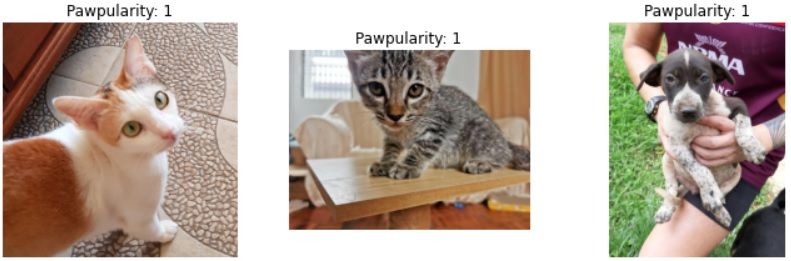
\includegraphics[scale=0.5]{Plot/pawpularity_1.jpg}
        \caption{Animali con Pawpularity=1}
        \label{fig:paw_10}
    \end{figure}

    \begin{figure}[H]
        \centering
        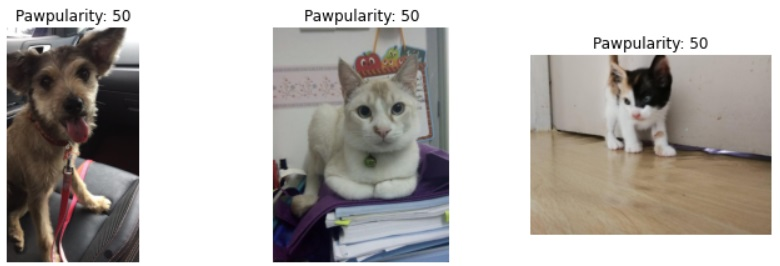
\includegraphics[scale=0.5]{Plot/pawpularity_50.jpg}
        \caption{Animali con Pawpularity=50}
        \label{fig:paw_50}
    \end{figure}

    \begin{figure}[H]
        \centering
        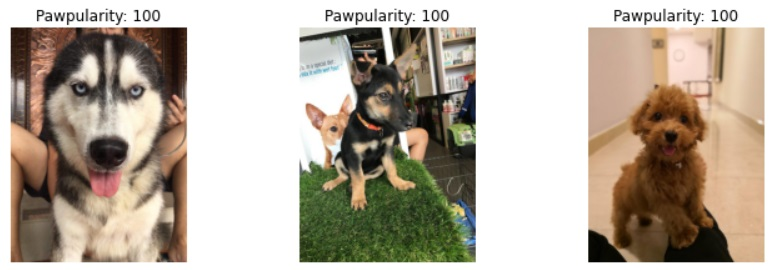
\includegraphics[scale=0.5]{Plot/pawpularity_100.jpg}
        \caption{Animali con Pawpularity=100}
        \label{fig:paw_100}
    \end{figure}

    Dall'analisi visiva effettuata non si evincono particolari dettagli su cosa possa rendere una foto più "popolare" rispetto ad un'altra, è facile, infatti, trovare delle belle foto di animali con score di pawpularity sotto il 10.

    \subsubsection{Metadati}
    Come descritto in precedenza il file \textit{train.csv} contiene i metadati per ogni immagine. In figura \ref{fig:target} visualizziamo la distribuzione del target, ovvero il Pawpularity score.
    \begin{figure}[H]
        \centering
        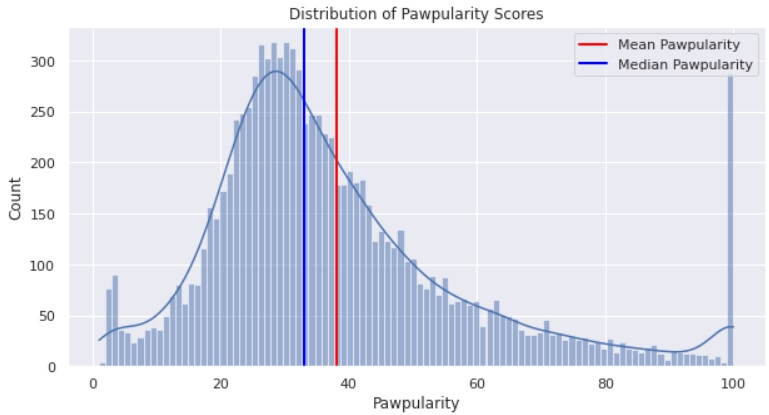
\includegraphics[scale=0.8]{Plot/distribution_target.jpg}
        \caption{Distribuzione e esempio della feature Focus}
        \label{fig:target}
    \end{figure}

    Osserviamo come la distribuzione dello score sia concentrata principalmente tra i valori 20 e 50. È facile osservare anche una forte presenza di immagini con score uguale a 100.
    Successivamente analizziamo la distribuzione del target per ogni singola feature del dataset.
    Per fare ciò usiamo degli istogrammi, plottiamo il Pawpularity score sull'asse x e la somma degli 0s e degli 1s di ogni feature sull'asse y. Questo ci può aiutare a visualizzare se alcune feature impattano più di altre nel calcolo del Pawpularity score. Per ogni feature inoltre vengono mostrati degli esempi di immagini per contestualizzare meglio il significato della feature stessa.

    \begin{itemize}
        \item \textbf{Focus} - L'animale è posizionato su uno sfondo ordinato, non troppo vicino/lontano;
        \begin{figure}[H]
            \centering
            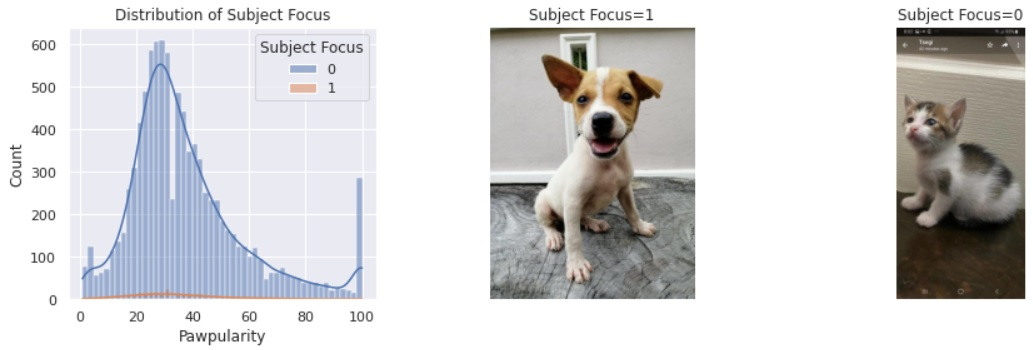
\includegraphics[scale=0.5]{Plot/distribution_subjectfocus.jpg}
            \caption{Distribuzione e esempio della feature Focus}
            \label{fig:focus}
        \end{figure}
        \item \textbf{Eyes} - Entrambi gli occhi sono rivolti verso l'obiettivo, con almeno un occhio/pupilla decentemente chiaro;
        \begin{figure}[H]
            \centering
            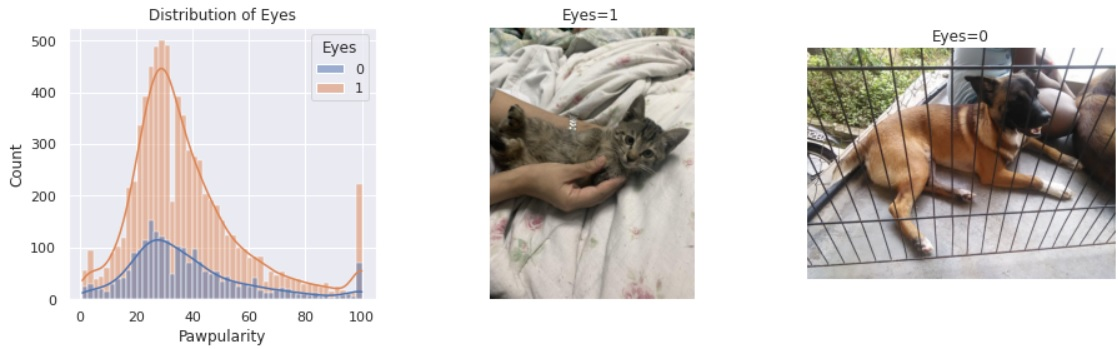
\includegraphics[scale=0.5]{Plot/distribution_eyes.jpg}
            \caption{Distribuzione e esempio della feature Eyes}
            \label{fig:eyes}
        \end{figure}
        \item \textbf{Face} - Viso discretamente chiaro e rivolto in avanti;
        \begin{figure}[H]
            \centering
            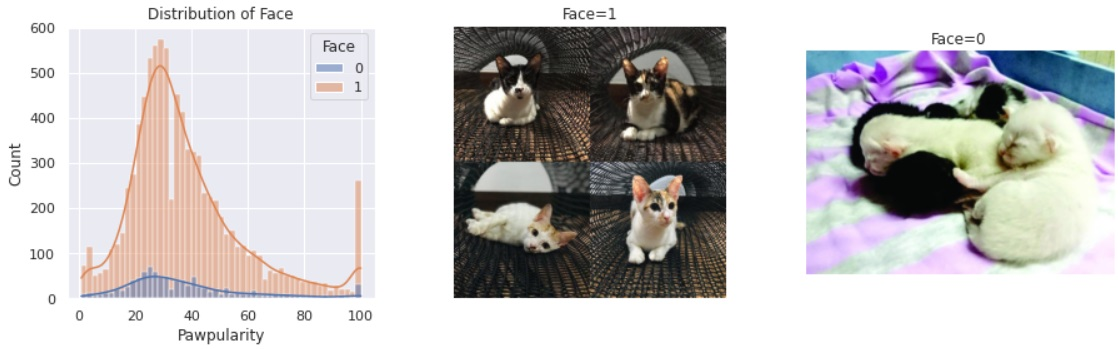
\includegraphics[scale=0.5]{Plot/distribution_face.jpg}
            \caption{Distribuzione e esempio della feature Face}
            \label{fig:face}
        \end{figure}
        \item \textbf{Near} - Singolo animale che occupa una porzione significativa della foto (circa oltre il 50\% della larghezza o dell'altezza della foto);
        \begin{figure}[H]
            \centering
            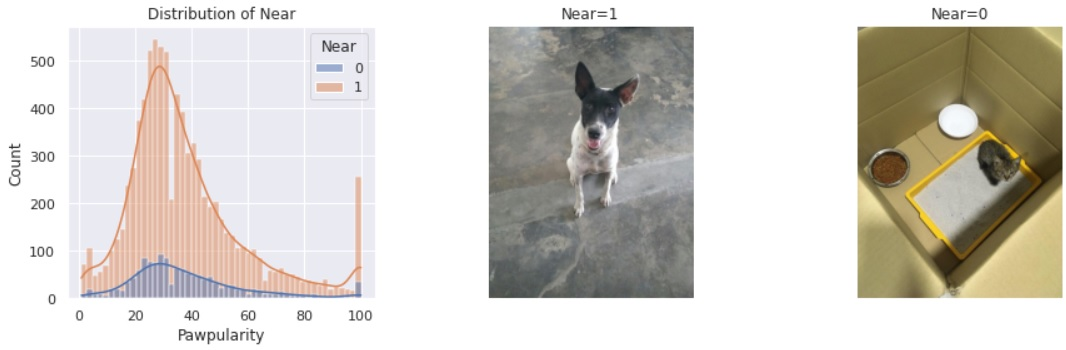
\includegraphics[scale=0.5]{Plot/distribution_near.jpg}
            \caption{Distribuzione e esempio della feature Near}
            \label{fig:near}
        \end{figure}
        \item \textbf{Action} - Animale nel mentre di un'azione (ad es. saltare);
        \begin{figure}[H]
            \centering
            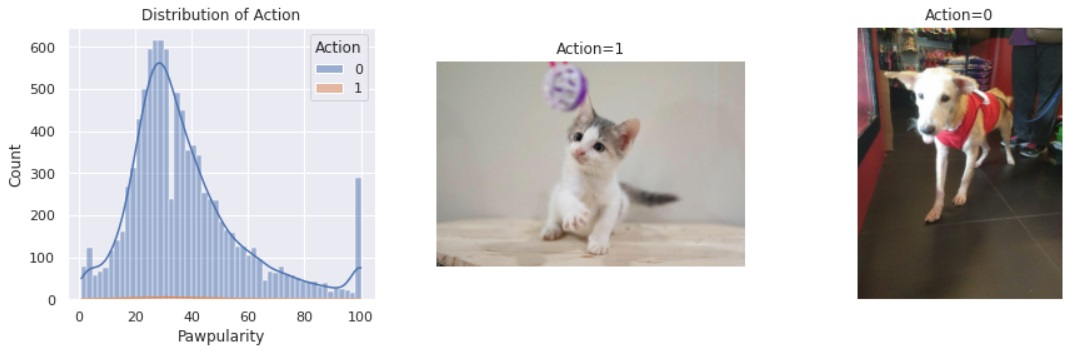
\includegraphics[scale=0.5]{Plot/distribution_action.jpg}
            \caption{Distribuzione e esempio della feature Action}
            \label{fig:action}
        \end{figure}
        \item \textbf{Accessory} - Accessorio/oggetto di accompagnamento fisico o digitale, come un giocattolo o un adesivo digitale, esclusi collare e guinzaglio;
        \begin{figure}[H]
            \centering
            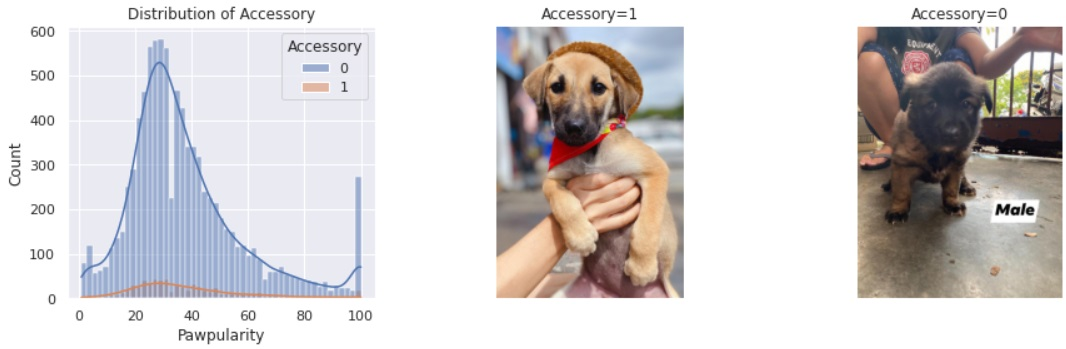
\includegraphics[scale=0.5]{Plot/distribution_accessory.jpg}
            \caption{Distribuzione e esempio della feature Accessory}
            \label{fig:accessory}
        \end{figure}
        \item \textbf{Group} - Più di 1 animale nella foto;
        \begin{figure}[H]
            \centering
            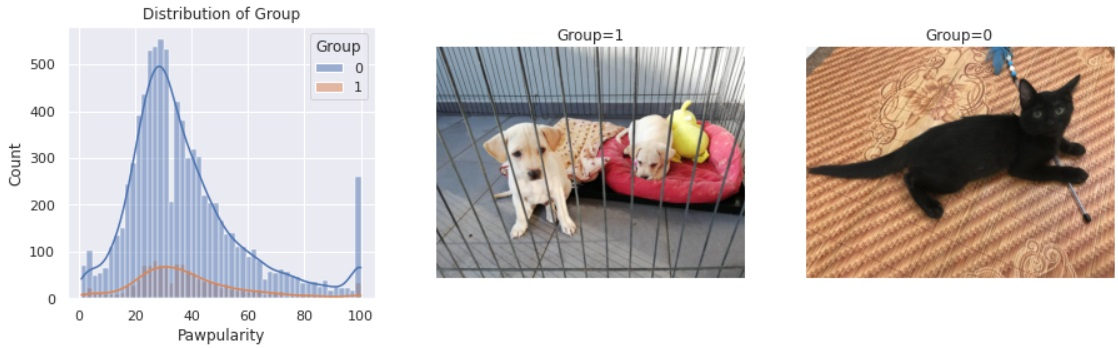
\includegraphics[scale=0.5]{Plot/distribution_group.jpg}
            \caption{Distribuzione e esempio della feature Group}
            \label{fig:group}
        \end{figure}
        \item \textbf{Collage} - Foto ritoccata digitalmente;
        \begin{figure}[H]
            \centering
            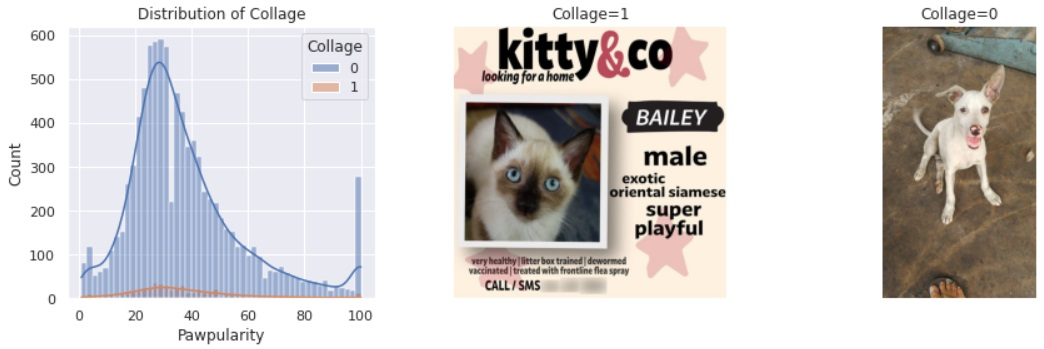
\includegraphics[scale=0.5]{Plot/distribution_collage.jpg}
            \caption{Distribuzione e esempio della feature Collage}
            \label{fig:collage}
        \end{figure}
        \item \textbf{Human} - Umano nella foto;
        \begin{figure}[H]
            \centering
            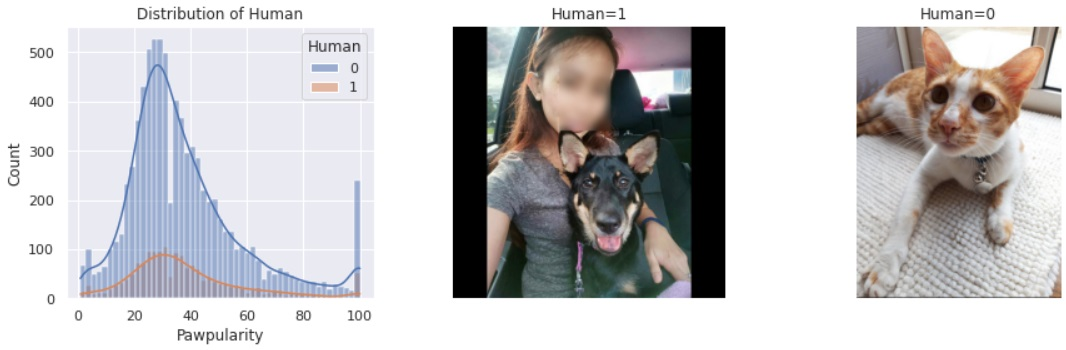
\includegraphics[scale=0.5]{Plot/distribution_human.jpg}
            \caption{Distribuzione e esempio della feature Human}
            \label{fig:human}
        \end{figure}
        \item \textbf{Occlusion} - Oggetti indesiderati che bloccano una parte dell'animale. Nota: Non tutti gli oggetti bloccanti sono considerati occlusione;
        \begin{figure}[H]
            \centering
            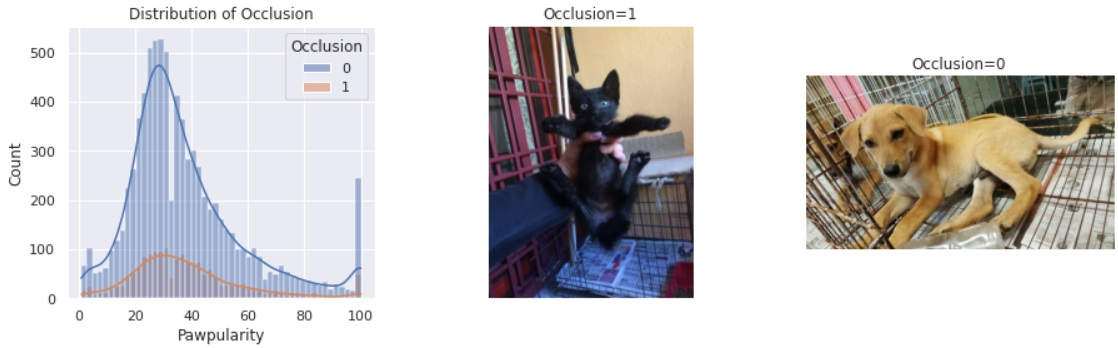
\includegraphics[scale=0.5]{Plot/distribution_occlusion.jpg}
            \caption{Distribuzione e esempio della feature Occlusion}
            \label{fig:occlusion}
        \end{figure}
        \item \textbf{Info} - Mesto o etichette personalizzati (ad es. nome dell'animale, descrizione);
        \begin{figure}[H]
            \centering
            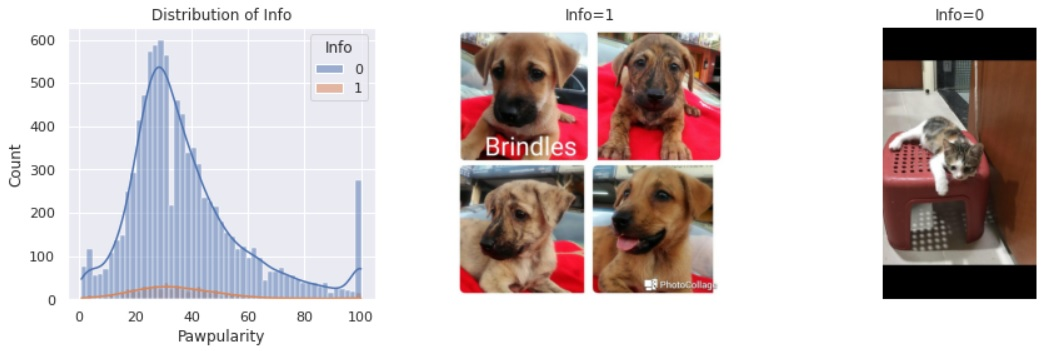
\includegraphics[scale=0.5]{Plot/distribution_info.jpg}
            \caption{Distribuzione e esempio della feature Info}
            \label{fig:info}
        \end{figure}
        \item \textbf{Blur} - Notevolmente sfocato o rumoroso, soprattutto per gli occhi e il viso dell'animale. Per le voci Sfocatura, la colonna "Occhi" è sempre impostata su 0.
        \begin{figure}[H]
            \centering
            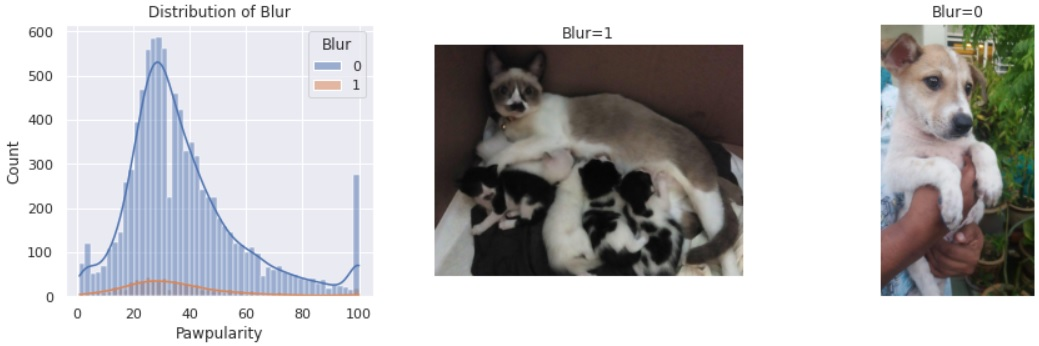
\includegraphics[scale=0.5]{Plot/distribution_blur.jpg}
            \caption{Distribuzione e esempio della feature Blur}
            \label{fig:blur}
        \end{figure}
    \end{itemize}
    
    Intuitivamente possiamo dire che questi grafici non ci dicono molto. La distribuzione del Pawpularity score è simile per ogni feature, in altre parole nessuna feature in particolare sembra influenzare particolarmente il Pawpularity score.
    \vfill

\section{The Methodological Approach}


    L'approccio proposto è basato su un modello multi-input single-output. La motivazione alla base di questo approccio è quella di sviluppare un sistema di apprendimento che sia in grado di sfruttare le informazioni utili da features miste di dati, poiché questi tipi di dati di solito richiedono un trattamento separato. A tal fine, ogni tipo di dato in ingresso viene elaborato e gestito in modo diverso e indipendente. L'architettura proposta è mostrata in figura \ref{fig:model}


    \begin{figure}[h!]
        \centering
        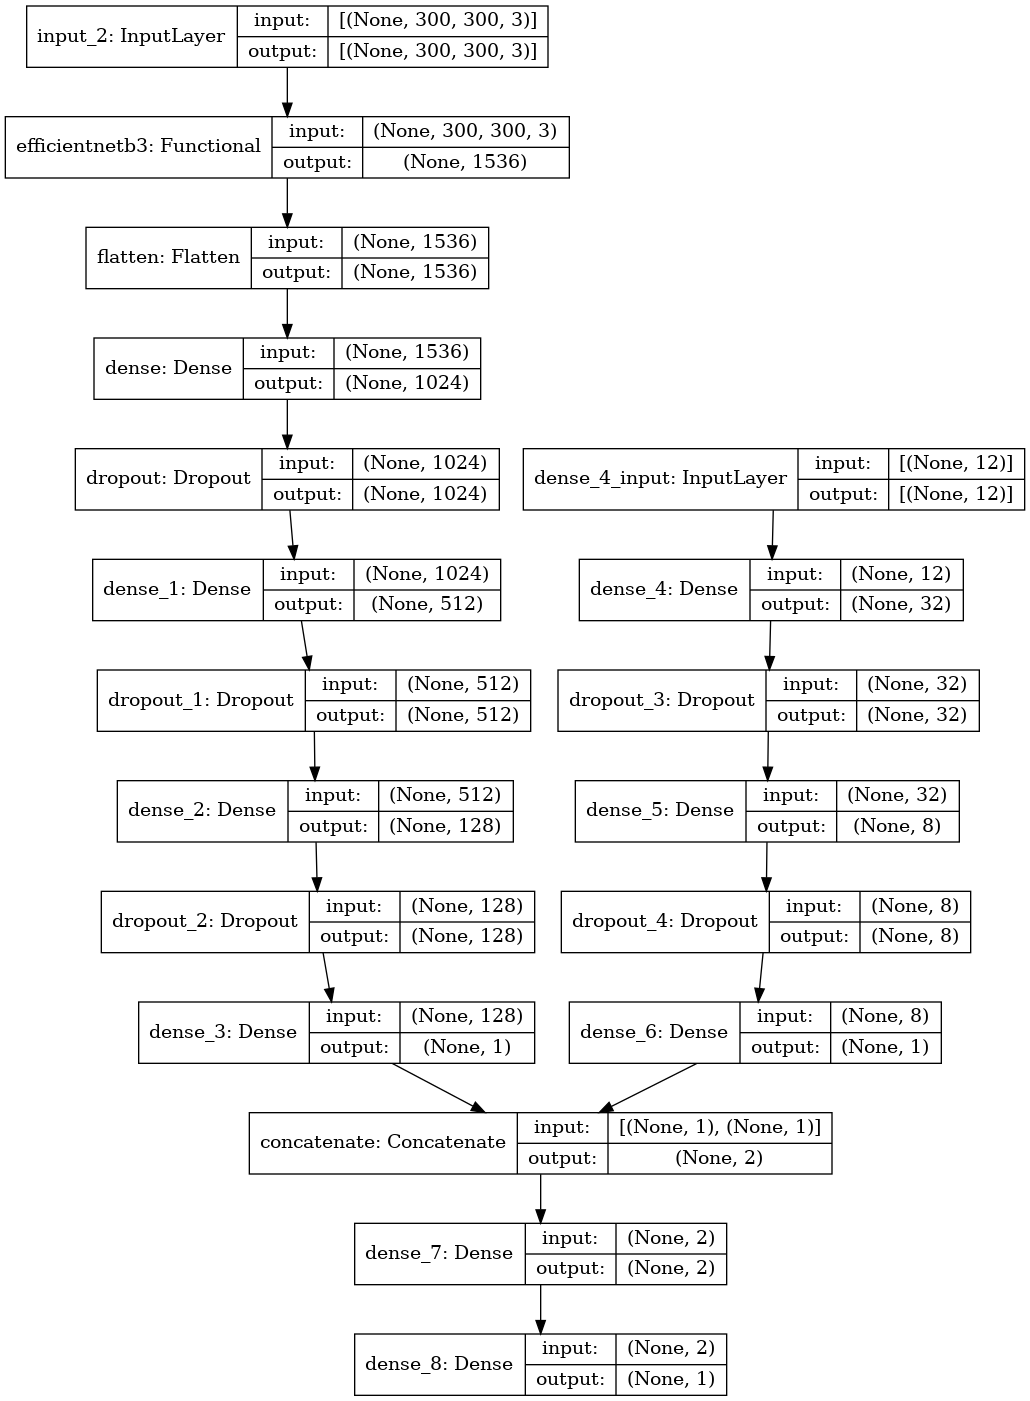
\includegraphics[scale=0.35]{Plot/Model-Plot.png}
        \caption{Multi-input Single-output Model}
        \label{fig:model}
    \end{figure}

\subsection{}

This is the central and most important section of the report. Its objective must be to show, with linearity and clarity, the steps that have led to the definition of a decision model. The description of the working hypotheses, confirmed or denied, can be found in this section together with the description of the subsequent refining processes of the models. Comparisons between different models (e.g. heuristics vs. optimal models) in terms of quality of solutions, their explainability and execution times are welcome. 

Do not attempt to describe all the code in the system, and do not include large pieces of code in this section, use pseudo-code where necessary. Complete source code should be provided separately (in Appendixes, as separated material or as a link to an on-line repo). Instead pick out and describe just the pieces of code which, for example:
\begin{itemize}
\item are especially critical to the operation of the system;
\item you feel might be of particular interest to the reader for some reason;
\item  illustrate a non-standard or innovative way of implementing an algorithm, data
structure, etc..
\end{itemize}

You should also mention any unforeseen problems you encountered when implementing the
system and how and to what extent you overcame them. Common problems are:
 difficulties involving existing software.


\section{Results and Evaluation}
The Results section is dedicated to presenting the actual results (i.e. measured and calculated quantities), not to discussing their meaning or interpretation. The results should be summarized using appropriate Tables and Figures (graphs or schematics). Every Figure and Table should have a legend that describes concisely what is contained or shown. Figure legends go below the figure, table legends above the table. Throughout the report, but especially in this section, pay attention to reporting numbers with an appropriate number of significant figures. 

\section{Discussion}
The discussion section aims at interpreting the results in light of the project's objectives. The most important goal of this section is to interpret the results so that the reader is informed of the insight or answers that the results provide. This section should also present an evaluation of the particular approach taken by the group. For example: Based on the results, how could the experimental procedure be improved? What additional, future work may be warranted? What recommendations can be drawn?


\section{Conclusions}
Conclusions should summarize the central points made in the Discussion section, reinforcing for the reader the value and implications of the work. If the results were not definitive, specific future work that may be needed can be (briefly) described. The conclusions should never contain ``surprises''. Therefore, any conclusions should be based on observations and data already discussed. It is considered extremely bad form to introduce new data in the conclusions.

\section*{References}

The references section should contain complete citations following standard form.  The references should be numbered and listed in the order they were cited in the body of the report. In the text of the report, a particular reference can be cited by using a numerical number in brackets as \cite{Lee2015} that corresponds to its number in the reference list. \LaTeX provides several styles to format the references

\bibliographystyle{IEEEtran}
\bibliography{references.bib}

\end{document}